\begin{figure}[!ht]
	\centering
	\subfigure[][Optical information]{\label{fig:visual_info}
	    \begin{minipage}[b]{0.44\linewidth}
   			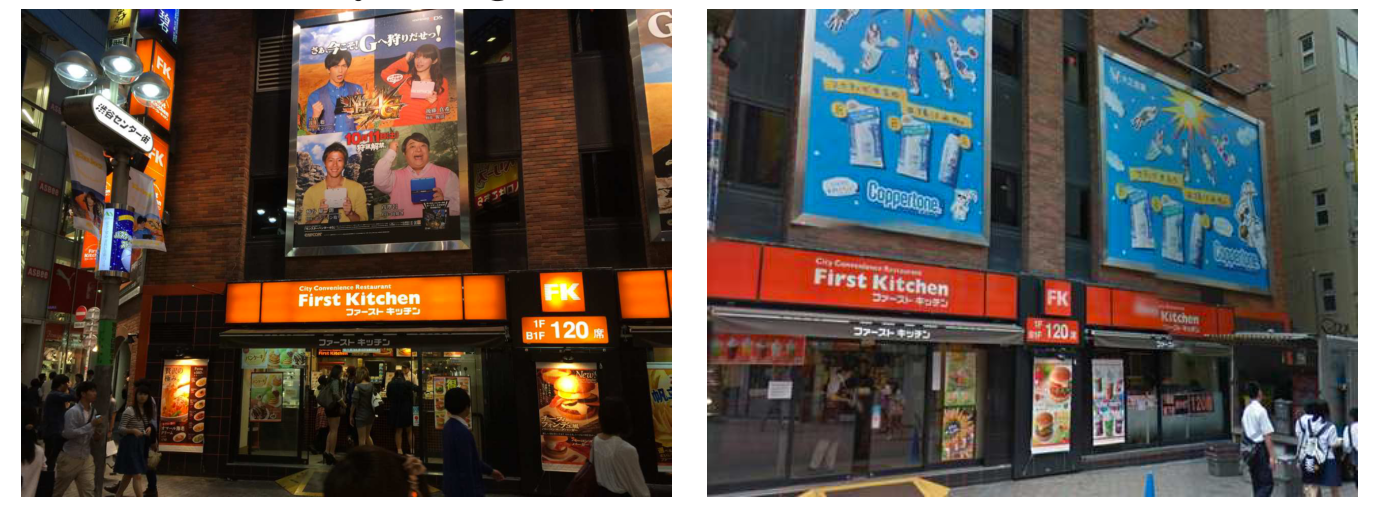
\includegraphics[width=\linewidth]{data_hetero/street_level_2.png}

			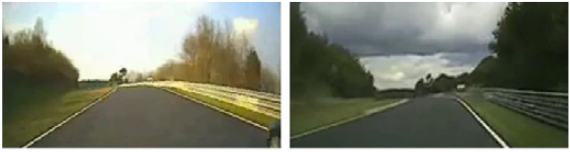
\includegraphics[width=\linewidth]{data_hetero/road.png}
	
			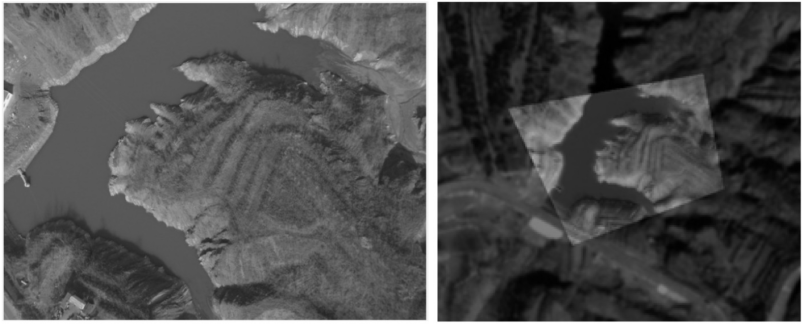
\includegraphics[width=\linewidth]{data_hetero/overhead.png}
	    \end{minipage}
	}
	\begin{minipage}[b]{0.55\linewidth}
   		\subfigure[][Geometric information]{\label{fig:3d_info}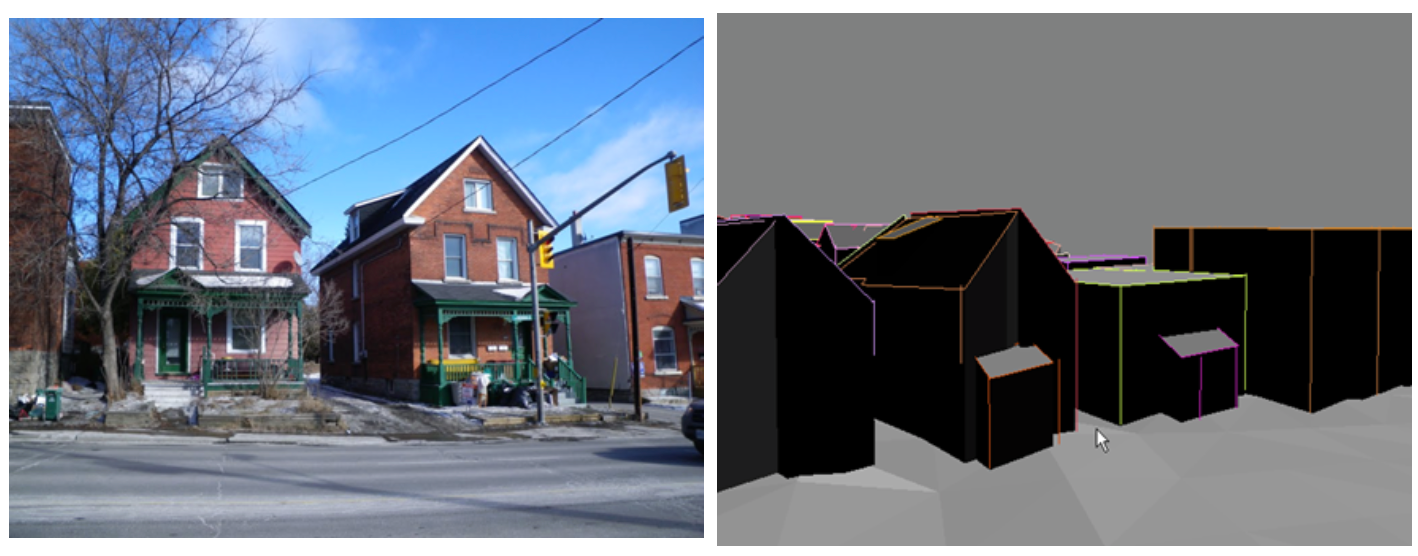
\includegraphics[width=\linewidth]{data_hetero/image_to_DEM.png}}
   		    
   		\subfigure[][Semantic information]{\label{fig:seg_ifo}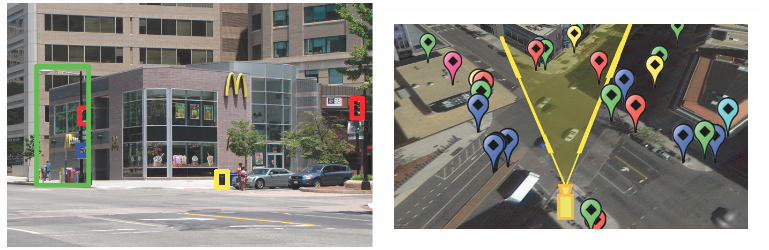
\includegraphics[width=\linewidth]{data_hetero/semantic.png}}
	\end{minipage}
	\caption[Illustration of the data heterogeneity in \ac{vbl}]{\textbf{Illustration of the data heterogeneity in \ac{vbl}:} \ref{fig:visual_info}~Image-based \ac{vbl} systems, left represent the query image and right the closest corresponding image in the database. Images appearance differ depending on the final application, from top to bottom:~street-level localization in urban environment from \citep{Torii2015}, car localization on road from \citep{Milford2012}, air-plane localization with aerial imagery from \citep{Wan2016}. \ref{fig:3d_info}~Localization system built upon a DEM from \citep{Matei2013}:~left represent the query image and right the closest corresponding pose according to the 3D model. \ref{fig:seg_ifo}~Localization system with semantic information integration from \citep{Ardeshir2014}:~on the left the query image with segmented objects (colour boxes) and on the right the retrieved pose (yellow camera) from a map with semantic objects location (coloured landmarks). \label{fig:data_div}}
\end{figure}